\documentclass[12pt]{article}
\usepackage{graphicx}
\usepackage{amsfonts,amssymb,amsmath} 
\usepackage{lmodern,adjustbox}
\usepackage{float}
\usepackage{subcaption}
\usepackage{comment}
\usepackage{physics}
\usepackage{tikz}
\usetikzlibrary{quantikz}
\usepackage{mathtools}
\usepackage[a4paper, left = 1.5cm, right = 1.5cm, top = 3.5cm, bottom = 3.5cm ]{geometry}
\usepackage{listings}
\usepackage{mathtools} 
\usepackage{extarrows} 


\newtheorem{definition}{Definition}[section]
\newtheorem{proof}{Proof}[section]

\begin{document}
	
	\begin{titlepage}
		
		\title{Self-Supervised Learning for pre-training models in Computer Vision \\ \vspace{1cm} Continual Learning Report}
		\author{Diego Arcelli}
		\maketitle
		\centering
		
\includegraphics[width=10cm]{./images/unipi_logo.png}
		
	\end{titlepage}
	
	\tableofcontents
	\newpage
	
	\begin{abstract}
	\noindent In this work some self-supervised learning methods for computer vision will be explored. In the first part the general framework of self-supervised learning will be discussed, describing all the aspects which are in common to the methods that will be explained. After that five different self-supervised learning methods will be described in detail and in the final part of the work those methods will be compared, both in term of performances and in the way they address some specific problems, exposing strengths and weaknesses of each method.
	\end{abstract}
	
	\section{Introduction}
	Self-Supervised Learning (SSL) is a particular machine learning technique that enables models to learn from unlabeled data by self-generating the labels from the input patterns, usually requiring the model to predict or reconstruct some aspect of the input. The main objective of SSL is to pre-train a model on a large dataset using these self-generated labels, which allows the model to learn a meaningful and useful representation of the input data. This pre-trained model can then be fine-tuned on downstream tasks with a smaller labeled datasets, hopefully leading to improved performance and faster convergence compared to training the model from scratch. By learning a useful representation of the input, the pre-trained model can extract relevant features and patterns that are beneficial for the downstream tasks, even if the labeled dataset is different from the original unlabeled dataset used for pre-training. SSL has the advantages of requiring less labeled data, which are usually hard to acquire, enabling to learn from unlabeled data, which are easier to get. Moreover the same pre-trained model might be used for many downstream tasks. 
	
	SSL gained a lot of popularity in the field of natural language process, where pre-training large language models on pretext tasks, such as masked language modeling or next sentence prediction, allowed to reach remarkable performances on many downstream tasks. In this work some techniques to perform SSL in computer vision scenarios will be analyzed, discussed and compared.
	
	\section{Problem setting}
	As explained in the previous section we will consider SSL for computer vision tasks. In general when we train a self-supervised model there are two main stages:
	\begin{itemize}
		\item[--] \textbf{Pretext task}: which is the self-supervised task that is used to pre-train the model. The goal of this task is to learn a good intermediate representation with the expectation that this representation can carry good semantic or structural meanings and can be beneficial for many downstream tasks.
		\item[--] \textbf{Downstream task}: which is the supervised task (such as image classification or object detection) on which we want to evaluate the model. In this stage the pre-trained model is used as a starting point, and the weights are adjusted through supervised training on the downstream task, using labeled data.
	\end{itemize}
	In general we don't care about the performances of the model in the pretext task, and we just care about the performances on the downstream tasks. When fine-tuning the model on the downstream task, usually a classifier (typically an MLP) is added at the end of the feature extractor learned during the pre-training, and it is trained to perform the supervised task. In general for the fine-tuning we can:
	\begin{itemize}
		\item[--] Train the parameters of the whole architecture
		\item[--] Freeze the parameters of the feature extractor and only train the weights of the MLP head
		\item[--] Freeze the parameters of the first $K$ layers of the feature extractor and train the weights of the rest of the architecture
	\end{itemize}
	All the methods that we'll explore exploit two fundamental concepts for SSL in computer vision: data augmentation and contrastive learning. As we already said in SSL we want to train a model using unlabeled data to predict some properties of the data. In the textual domain this is usually done by masking some words in a sentence and training the model to predict those words. In computer vision one possible way of doing is by taking an image, producing different views of that image by applying to each view a different set of transformations, and consider views produced from the same image to belong to the same class. In this way we can train a model that takes in input two views to predict if they come from the same image or not. We define a couple of images to be a positive pair if they are different views of the same image, on the contrary we define the couple as a negative pair if the two images are views from different images. If we merge this idea of positive and negative pairs obtained with data augmentation, with the goal that we want to achieve with the pretext task, which is learning a latent representation of the images that carry semantic information of the images, we get the intuition is that the in the latent space two positive images should be close, while two negative images should be distant. This is the intuition behind contrastive learning, in which we train a model to produce a representation of the data using a loss the minimize in the latent space the distance between positive images and maximize the distance between negative images.
	
	
	\section{Methodology}
	
	\subsection*{Contrastive Predicting Coding}
	Contrastive Predictive Coding (CPC) \cite{oord2018representation} is a method which has been thought actually not only for the computer vision field, but it can be applied also to other domains like audio and natural language. The idea of the method is to train a model that learns representation of the data by predicting the representation of future observations from the past ones. When applied to image processing CPC works as follows: from an image we extract a certain number of overlapping crops of a fixed size and we organize those crops in a grid. If $x_{i,j}$ is the crop in position $i, j$ of the grid, then we use an encoder $f_\theta(\cdot)$ to encode each crop of the grid into a single vector $z_{i,j} = f_\theta(x_{i,j})$. After that a second auto-regressive model $g_\phi(\cdot)$ is used to compute $c_{i,j} = g_\phi(\{z_{u,v}\}_{u\le i, v})$ that is a context vector that summarizes the feature in the previous rows but in the same column of $z_{i,j}$. The predictive tasks consists of predicting a feature vectors $z_{i+k,j}$ from the context vector $c_{i,j}$, where $k > 0$, using a linear model $W_k$ computing $\hat{z}_{i+k,j} = W_kc_{i,j}$. To measure the quality of the prediction a contrastive loss is employed:
\[ \mathcal{L}_{\text{CPC}} = -\sum_{i,j,k}\log p(z_{i+k,j}|\hat{z}_{i+k,j}, \{z_l\}) = -\sum_{i,j,k}\log \frac{\exp(\hat{z}^T_{i+k,j}z^T_{i+k,j})}{\exp(\hat{z}^T_{i+k,j}z^T_{i+k,j}) + \sum_l \exp(\hat{z}^T_{i+k,j}z^T_l)}\]
where $\{z_l\}$ is the set of negative samples which is composed by taking crops from different location of the grid. In the paper they prove formally that minimizing this loss is equivalent of maximizing the mutual information between $c_{i,j}$ and $x_{i+k,j}$, obtaining the bound:
\[ I(x_{i+k,j}, c_{i,j}) \ge \log(N) - \mathcal{L}_{CPC}\]
where $N$ is the number of negative examples used in the loss. After having trained the whole architecture, for the fine-tuning on downstream tasks we keep only the encoder network $f_\theta(\cdot)$ and use it as feature extractor for a classification model, which is then trained on a supervised task  For the encoder $f_\theta$ any CNN can be applied, in the paper the authors used a ResNet101, while for the auto-regressive model $g_\phi$ they used a PixelCNN.

In \cite{henaff2020data} the authors proposes CPC-v2, an improved version of CPC where essentially they do some modification of some training details like applying augmentation to the crops individually, increasing the crops sizes, using layer normalization instead of batch normalization and some other minors modifications, but the backbone of the method remains the same.
	
	\subsection*{Contrastive Multi-view Coding}
	In Contrastive Multi-view Coding (CMC) \cite{tian2020contrastive} the authors start from the framework proposed in CPC, but they adapt it to maximize the mutual information between different views of the same image, removing the prediction part and focusing on contrastive learning. Suppose we have two different views of a dataset $V_1$ and $V_2$, and we build a dataset that consist of a collection of samples $\{v_1^i, v_2^i\}_{i=1}^N$. We consider positive pairs those which are sampled from the joint distribution $x \sim p(v_1, v_2)$ where $x= \{v_1^i, v_2^i\}$, while we consider negative samples those sampled from the product of marginals $y \sim p(v_1)p(v_2)$ where $y = \{v_1^i, v_2^j\}$. The goal is to learn a critic function $h_\theta$ which is trained to output high values for positive pairs and low values for negative pairs. In this way we can use a contrastive loss function that we can use to train the model to correctly select a single positive sample out of a set that contains $k$ negative samples:
\[\mathcal{L}^{V_1, V_2}_{contrast} = -\mathbb{E}_{\{v_1^1, v_2^1, \dots, v_2^{k+1}\}} \Bigg[ \log \frac{h_\theta(\{v_1^1, v_2^1 \})}{\sum_{j=1}^{k+1}h_\theta(\{v_1^1, v_2^j \})}  \Bigg] \]
where $\{v_1^1, v_2^1 \}$ is the positive pair and $\{v_1^1, v_2^j \}$ with $j > 1$ is the a negative pair. To extract the latent representations of $v_1$ and $v_2$ we use two encoders $f_{\theta_1}(\cdot)$ and $f_{\theta_2}(\cdot)$. We compute the latent representations $z_1 = f_{\theta_1}(v_1)$ and $z_2 = f_{\theta_1}(v_2)$ which we can use to compute the output of the critic as:
\[ h_\theta(\{v_1, v_2\}) = \text{exp}\Bigg(\frac{z_1^Tz_2}{\lVert z_1\rVert \lVert z_2\rVert}\cdot \frac{1}{\tau}\Bigg) \]
In the formulation of $\mathcal{L}^{V_1, V_2}_{contrast}$ the view $V_1$ is used as anchor view, while we enumerate samples from view $V_2$, but we can also do the opposite and use the following loss:
\[ \mathcal{L}(V_1, V_2) = \mathcal{L}^{V_1, V_2}_{contrast} + \mathcal{L}^{V_2, V_1}_{contrast} \]
After the training phase, if we want for instance to fine-tune the model on an image classification task, we can concatenate the output of the two encoder networks $f_{\theta_1}$ and $f_{\theta_2}$ and use it as input of a classification network.
In the paper the authors prove that the optimal critic $h^*_\theta$ is proportional to the density ratio between the joint distribution $p(z_1, z_2)$ and the product of the marginals $p(z_1)p(z_2)$:
\[ h^*_\theta(\{ v_1,v_2\}) \propto \frac{p(z_1, z_2)}{p(z_1)p(z_2)} \propto \frac{p(z_1|z_2)}{p(z_1)} \]
that is the point-wise mutual information and from this the same bound obtained for CPC can be derived:
\[I(z_i;z_j) \ge \log(k) - \mathcal{L}_{contrast} \]
hence minimizing the contrastive loss yields to the maximization of the mutual information between the latent representation of the different views.\\
Then the authors proposes two different ways for extending the this framework to the usage of multiple views. Suppose we have $M$ different views of a dataset $V_1, \dots, V_M$, we can extend CMC to the multiple views case using the following losses:
\[ \mathcal{L}_C = \sum_{j=2}^{M} \mathcal{L}(V_1, V_j), \qquad \mathcal{L}_F = \sum_{j=1}^{M} \sum_{i=1}^{j-1} \mathcal{L}(V_i, V_j)\]
in the core view formulation ($\mathcal{L}_C$) we select one view that we want to optimize, for instance $V_1$, and we build a pairwise representations between $V_1$ and all the other views. In the full graph formulation ($\mathcal{L}_F$) we instead consider all the possible pairs. The full graph formulation is more computational expensive but it has the advantage that it allows to capture more information between different views.\\
In order to achieve good results using many negative examples in the contrastive loss, CMC uses a memory bank to store latent representations for each training sample, so that a certain amount of negative samples can be retrieved from the memory bank without recomputing the features each time. The drawback of course is the fact the representations in the memory becomes old after some time and they must be updated after some time.\\
In the experiments in order to produce different views of the images, they convert the images from the RGB to the Lab representation, and then they split each image into L and ab channels. Of course L and ab from the same image are considered positive pairs. They do the same thing for the YDbDr color space, splitting the Y and DbDr channels. For testing the multi-views case they again use the Lab representation separating the L and ab channels, and they also include other three views depth, surface normal and semantic labels (example in figure \ref{fig:cmc-views}).
\begin{figure}[H]
	\centering
	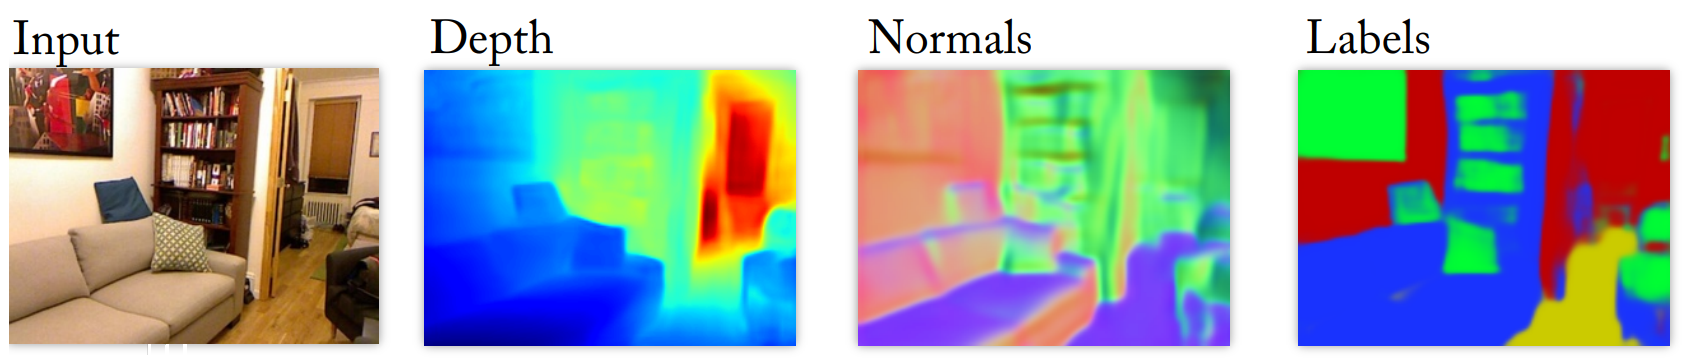
\includegraphics[width=10cm]{./images/cmc-views.png}
	\caption{Example of depth, normal and semantic labels views of an image}
	\label{fig:cmc-views}
\end{figure}

	
	\subsection*{Pre-text Invariant Representation Learning}
	Pre-text Invariant Representation Learning (PIRL) \cite{misra2020self} is a SSL method that uses contrastive learning like CMC, but the intention of the author is to train a model which learn a representation of the input images that is invariant with respect to image transformations.
\begin{figure}[H]
	\centering
	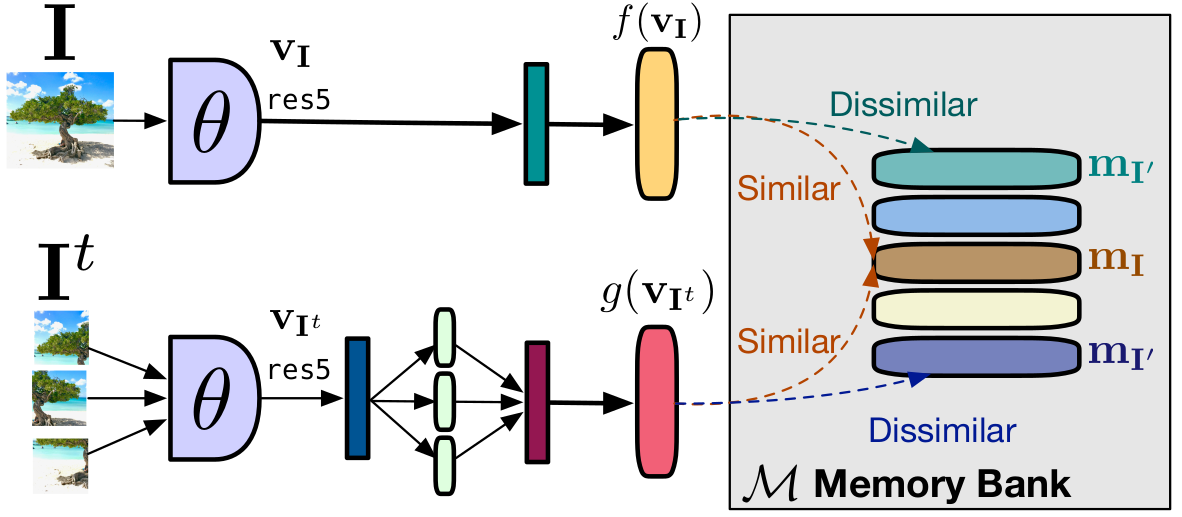
\includegraphics[width=8cm]{./images/pirl_scheme.png}
	\caption{Scheme that shows how PIRL works}
	\label{fig:pirl_scheme}
\end{figure}
\noindent Given a dataset of images $\mathcal{D} = \{I_1, \dots ,I_{|D|}\}$ where $I_n \in \mathbb{R}^{H\times W\times3}$ and set of transformation $\mathcal{T}$, the goal of PIRL is to train a convolutional neural network $\phi_\theta(\cdot)$ that constructs image representations $v_I = \phi_\theta(I)$ which are invariant to image transformations in $\mathcal{T}$. In order to do so $\phi_\theta$ is trained to minimize the following loss function:
\[ \ell_{inv}(\theta;\mathcal{D}) = \mathbb{E}_{t \sim p(\mathcal{T})}\Bigg[ \frac{1}{|D|} \sum_{I \in \mathcal{D}} L(v_I, v_{I^t}) \Bigg] \]
where $I^t = t(I)$ is the image $I$ after transformation $t$,  $L(\cdot, \cdot)$ measures the similarity between two image representations and $p(\mathcal{T})$ is a distribution over the transformation in $\mathcal{T}$. Minimization of this loss encourages the network $\phi_\theta(\cdot)$ to produce the same representation for the image $I$ as the transformed counter part $I^t$, so to make the representation invariant with respect to transformation $t$. This is in contrast to other losses of the following form:
\[ \ell_{cov}(\theta;\mathcal{D}) = \mathbb{E}_{t \sim p(\mathcal{T})}\Bigg[ \frac{1}{|D|} \sum_{I \in \mathcal{D}} L_{co}(v_I, z(t)) \Bigg] \]
where $z$ is a function that measures some property of the transformation $t$. These kind of losses push the network $\phi_\theta(\cdot)$ to make the representation covariant with respect to the transformation, which causes the network to learn information that are not semantically relevant.
$L(\cdot, \cdot)$ is defined as a contrastive loss:
\[h(v_I, v_{I^t}) = \frac{ \exp\Big(s(v_I, v_{I^t})/\tau \Big)}{ \exp\Big(s(v_I, v_{I^t})/\tau\Big) + \sum_{I^\prime \in \mathcal{D}_N}\exp\Big(s(v_I, v_{I^\prime})/\tau\Big)}\]
where $\mathcal{D}_N \subseteq \mathcal{D} \setminus \{I\}$ is a set of negative samples and $s(\cdot, \cdot)$ is a similarity function. Actually to compute the similarity we do not compute the features $v$ directly but we apply different heads. Specifically we use $f(\cdot)$ for $v_I$ and $g(\cdot)$ for $v_{I^t}$. So the actual loss is:
\[L_{\text{NCE}}(I, I^t) = -\log\big(h(f(v_I), g(v_{I^t}))\big) - \sum_{I^\prime \in \mathcal{D}_N} \log\big(1 - h(g(v^t_I), f(v_{I^\prime}))\big) \]
which encourages the representation of image $I$ to be similar to the one of its transformed counterpart $I^t$, while also encouraging it to be dissimilar to the representation of other images $I^\prime$.\\
To address the problem of finding many negative samples during the training the authors decided to use a memory bank $\mathcal{M}$ that contains the feature representation $m_I$ of image $I \in \mathcal{D}$. $m_I$ is an exponential moving average of the feature representation $f(v_I)$ that were computed in the prior epochs. In this way we can replace in the loss definition the negative samples $f(v^\prime_I)$ by their memory bank representation $m_{I^\prime}$, while keeping the batch size small. All the representation that are stored in the memory bank are all computed on the original images, $I$, without the transformation $t$. An issue of $L_{\text{NCE}}$ is that it does not compare the representation of the original image $I$ with the representation of the negative samples $I^\prime$, and this is fixed by using the following loss instead:
\[ L(I,I^t) = \lambda L_{\text{NCE}}(m_I, g(v_{I^t})) + (1-\lambda)L_{\text{NCE}}(m_I, f(v_I)) \]
where the first term is the one we had before and the second term encourages the representation of $f(v_I)$ to be similar to its memory bank representation $m_I$ and it also encourages the representation of $f(v_I)$ and $f(v_{I^\prime})$ to be dissimilar.
In practice the authors used a ResNet to compute the representation of the images. The difference between the two heads $f$ and $g$ is that for $g(v_{I^t})$ they extract 9 patches from the image, for each patch they compute the representation using the network, the representation of the patched are concatenated and passed to a linear projection which produces a 128-dimensional vector. The authors justify this decision by saying that they wanted to remain as close as possible to other covariant pretext tasks (like the Jigsaw), in order to have a fair comparison between the covariant approaches and their invariant approach.

	
	\subsection*{Momentum Contrast}
	Momentum Contrast (MoCo) \cite{he2020momentum} uses a prospective of contrastive learning as dictionary look-up. If we consider and encoded query $q$ and a and encoded set of of keys of the dictionary $\{k_1, k_2, \dots\}$ and we assume that there exists a single key $k_+$ that matches with $q$, we can define a contrastive loss ass a function that is low when $q$ is similar to its positive key $k_+$ and dissimilar to all the other negative keys. Specifically in the paper they use the InfoNCE loss: 
\[ \mathcal{L}_q = - \log\Bigg( \frac{\exp(q^Tk_+/\tau)}{\sum_{i=0}^K \exp(q^T k_i/\tau)}\Bigg)\]
that can be used as an unsupervised objective function for training the encoder networks that represent the queries and the keys: $q = f_q(x^q)$ and $k = f_k(x^k)$. Under this dictionary lookup prospective, contrastive learning is a way for building a discrete dictionary on high dimensional continuous inputs. This dictionary is dynamic since the keys are randomly sampled and $f_k(\cdot)$ changes during training.\\
Instead of using a memory bank like the ones of CMC and PIRL, MoCo maintains a queue of mini-batches of data samples. In this way the encoded keys from the preceding mini-batches can be used in the loss: at each training step the current mini batch is inserted in the queue and the oldest mini-batches is removed from the queue. The problem of using a large queue as a dictionary can be the update of the key encoder using back propagation intractable, since the gradient should propagate to all the samples in the queue, so the authors solve this problem by updating $f_k$'s parameters $\theta_k$ as a moving average of $f_q$'s parameters $\theta_q$:
\[\theta_k \leftarrow m\theta_k + (1-m)\theta_q \]
where $m \in [0,1)$. $\theta_q$ is normally updated using back-propagation. In this way $\theta_k$ evolves more smoothly than $\theta_q$, so even if the keys in the queue are encoded by different encoders, the difference between these encoders can be made small.\\
MoCo has been improved in a successive work \cite{chen2020simple} in which the authors applied to it some of the improvement proposed by SimCLR, which are a stronger data augmentation and the use of a MLP projection head after having computed the representation of the images using the encoder networks.
	
	\subsection*{Swapping Assignments between Multiple Views}
	Swapping Assignments between Multiple Views (SWAV) \cite{caron2020unsupervised} unlike all the other methods we've seen, it does not use contrastive learning but it is an online clustering based method. In clustering based method the idea is to use a clustering algorithm to cluster the embedding of a batch of images, and use those embedding as pseudo-label for a predictive task in which a model given the embedding of the images is trained to predict the cluster of each image. This method was proposed in Deep Cluster \cite{caron2018deep}.
\begin{figure}[H]
	\centering
	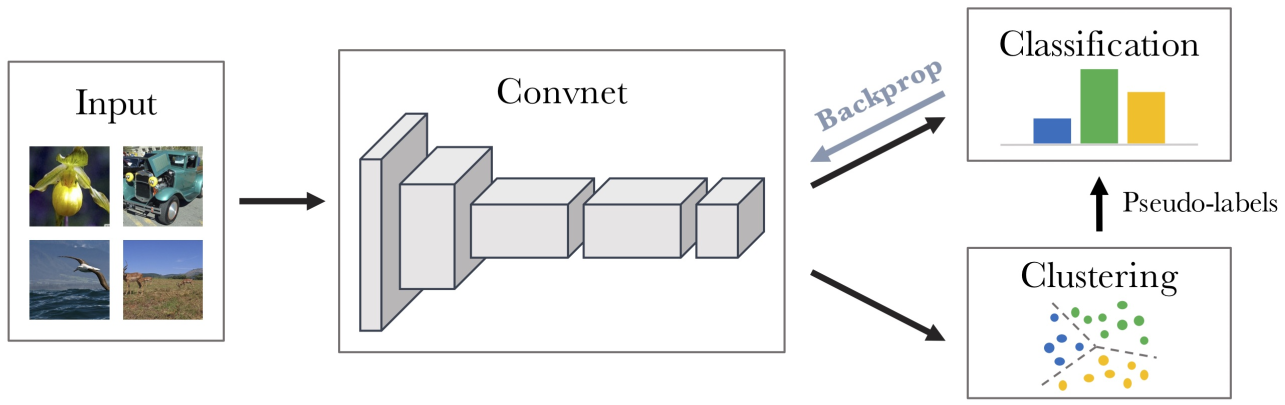
\includegraphics[width=10cm]{./images/deep_cluster.png}
	\caption{General framework of clustering based methods}
\end{figure}

With SWAV the authors combine the main framework of contrastive learning, which is comparing different views of the images produced with augmentation, with a clustering based pretext task. SWAV works as follows: each image $x_n$ is transformed into an augmented view $x_{nt}$ by applying a transformation $t \sim \mathcal{T}$, where $\mathcal{T}$ is a set of augmentations. Then we map the augmented view to a vector representation with a non-linear mapping $f_\theta$ to $x_{nt}$ and we then project this feature in a unit sphere $z_{nt} = f_\theta(x_{nt})/\lVert f_\theta(x_{nt}) \rVert_2$. From this representation we compute the code $q_{nt}$ by mapping $z_{nt}$ to a set of $K$ trainable prototypes vectors $\{c_1, \dots, c_k\}$. We use $C$ to denote the matrix whose columns are the $c_1, \dots, c_k$ vectors. If we do the same thing with another augmentation $s \sim \mathcal{T}$, obtaining the image feature $z_{ns}$ and its corresponding code $q_{ns}$ then we can set a swapped prediction problem using the following loss:
\[ L(z_{nt}, z_{ns}) = \ell(z_{nt}, q_{ns}) + \ell(z_{ns}, q_{nt}) \]
where the function $\ell(z, q)$ measures the fit between features $z$ and the code $q$. The idea is that instead of comparing directly the features of $z_t$ and $z_s$, we do it using the intermediate codes $q_t$ and $q_s$. If these two features capture the same information, it should be possible to predict the code of the feature $z_q$ using the feature $z_t$ and vice versa. The loss $\ell(z_t, q_s)$ is the cross entropy loss between the code and the probability obtained by taking a soft-max of the dot product of $x_i$ and all the prototypes in $C$:
\[\ell(z_t, q_s) = -\sum_k q_s^{(k)}\log p_t^{(k)}, \qquad p_t^{(k)} = \frac{\exp(z_t^Tc_k/\tau)}{\sum_{k^\prime}\exp(z_t^Tc_k^\prime/\tau)}\]
by applying some mathematical manipulations to these formula we can obtain our objective: 
\[\frac{1}{N}\sum_{n=1}^N \sum_{s, t \sim \mathcal{T}}L(z_{nt}, z_{ns}) = -\frac{1}{N}\sum_{n=1}^N \sum_{s, t \sim \mathcal{T}} \Bigg[ \frac{1}{\tau}z_{nt}^TCq_{ns} + \frac{1}{\tau}z_{ns}^TCq_{nt} - \log\sum_{i=1}^K\exp\Big(\frac{z_{nt}^Tc_k}{\tau}\Big) - \log\sum_{i=1}^K\exp\Big(\frac{z_{ns}^Tc_k}{\tau}\Big) \Bigg] \]
so we can train the parameters $\theta$ of the encoding function $f_\theta(\cdot)$ to minimize this loss.
\begin{figure}[H]
	\centering
	\subcaptionbox{Contrastive learning framework}
	{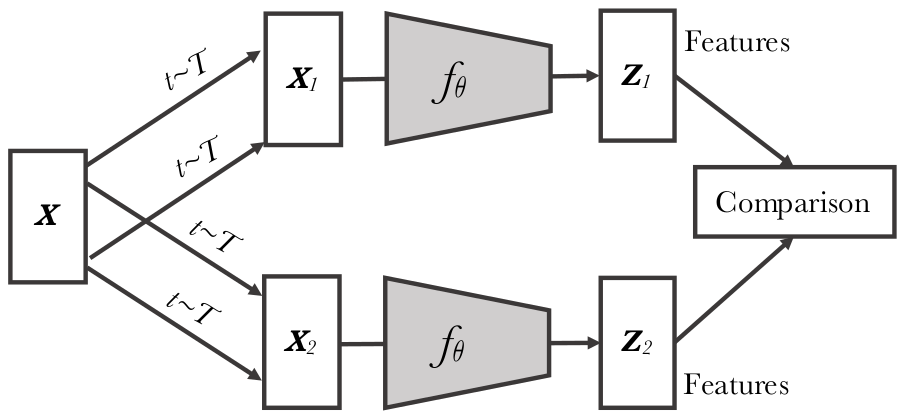
\includegraphics[width=0.4\textwidth]{./images/swav_contrastive.png}}
	\qquad
	\subcaptionbox{SWAV framework}
	{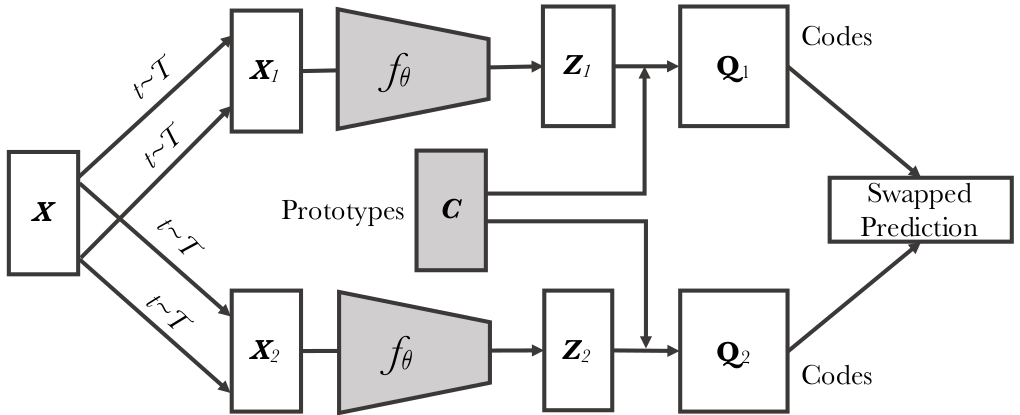
\includegraphics[width=0.4\textwidth]{./images/swav_prediction.png}}
	\caption{Difference between the classical contrastive learning framework with the one proposed in SWAV}

\end{figure}
The question now is how do we compute the codes? Given a batch of $B$ features $Z = [z_1, \dots, z_B]$ we want to map them to the prototypes $C= [C_1, \dots, C_K]$, obtaining the codes $Q = [q_1, \dots, q_B]$, where $Q$ is an $K\times B$ matrix where $Q_{i,j}$ can be viewed as the probability of feature $z_j$ to belong to the prototype $c_i$. We want to optimize $Q$ to maximize the similarity between features and prototypes, and this can be expressed in the following maximization problem:
\[ \max_{Q \in \mathcal{Q}} \Big\{ \Tr(Q^TC^TZ) + \epsilon H (Q) \Big\}\]
where $H(Q) = -\sum_i \sum_j Q_{i,j}\log Q_{i,j}$ and $\epsilon$ is a parameter that controls the smoothness of the mapping. The matrix $C^TZ$ contains the similarity of each feature vector and each prototype, since $(C^TZ)_{i,j} = c_i^Tz_j$.
%Hence we can r
%\[ \Tr(Q^TC^TZ) =  \sum_{i=1}^B\sum_{j=1}^K q_{j,i}(c^T_jz_i) = \sum_{i=1}^B\sum_{j=1}^K q_{j,i}\Big(\sum_{t=1}^Dc_{j,t}z_{i,t}\Big) \]
While solving the problem we need to avoid the trivial solution in which all the features are mapped to the same code. This can be achieved by imposing an equipartition constraint, which is basically saying that the number of feature vectors which are mapped to a given prototype has to be more or less the same for all the prototypes. In order to enforce the equal partitioning constraint the set $\mathcal{Q}$ is defined as:
\[ \mathcal{Q} = \{Q \in \mathbb{R}^{K \times B} | Q1_B = \frac{1}{k}1_k, Q^T1_K = \frac{1}{B}1_B \} \]
where $1_K$ denotes the $K$-dimensional vector where all the elements are 1. The solution to the optimization problem can be computed as:
\[ Q^* = \text{Diag}(u)\text{exp}\Big(\frac{C^TZ}{\epsilon}\Big)\text{Diag}(v) \]
where $u$ and $v$ are re-normalization vectors in $\mathbb{R}^K$ and $\mathbb{R}^B$, which can be computed with the Sinkhorn-Knopp algorithm.

	
	
	\section{Analysis and comparison}
	In this section the five methods we have explained will be compared in term of performances on different downstream tasks. In addition two other methods which have been explored during the lectures will be considered, SimCLR \cite{chen2020simple} and BYOL \cite{grill2020bootstrap}. As we already said in the previous sections, the way in which we evaluate SSL methods is by evaluating how downstream tasks perform after the SSL phase. Of course the evaluation on the downstream task might depends by many factors: the chosen dataset, the network used for the encoding, the hyper-parameters used for the methods the type of augmentations applied and so on. In this section I tried to use the results taken from the papers of the considered methods, from survey \cite{technologies9010002} and from this paper \cite{ericsson2021well}. In order to have a fair comparison I tried to collect results when the methods have been compared with the same encoder, and I also compared the methods on different datasets.

\noindent In table \ref{tab:imagenet-top1-5-acc-comp} we report the top-1 and top-5 accuracy of the considered methods when tested for classification on the ImageNet dataset and also the performances of a supervised model trained directly without SSL. All the methods uses as feature extractor a ResNet50 and the fine-tuning the SSL model is frozen and we train a linear classifier. PIRL, CPC are the two worst models while CMC does slightly better, SWAV and BYOL are by far the two best performing models, even if they do not reach the top-1 accuracy of the supervised model. MoCo and SimCLR are quite better than PIRL, CPC and CMP, but not as good as BYOL and SWAV.
\begin{table}[H]
	\centering
	\begin{tabular}{|l|l|cc|}
		\hline
		\multicolumn{1}{|c|}{\textbf{Method}} & \textbf{Architecture} & \multicolumn{2}{c|}{\textbf{ImageNet}} \\
		\multicolumn{1}{|c|}{} &  & Top1 & Top5 \\
		\hline
		Supervised & ResNet50 & 76.5 & - \\
		\hline
		PIRL & ResNet50 & 63.6 & - \\
		CPCv2 & ResNet50 & 63.8 & 85.3 \\
		CMC & ResNet50  & 66.2 & 87 \\
		SimCLR & ResNet50 & 69.3 & 89.0 \\
		MoCov2 & ResNet50 & 71.1 & - \\
		BYOL & ResNet50  & 74.3 & 91.6 \\ 
		SwAV & ResNet50 & 75.3 & - \\
		\hline
\end{tabular}
	\caption{Accuracy of the SSL methods using linear probing for fine-tuning}
	\label{tab:imagenet-top1-5-acc-comp}
\end{table}


Table \ref{tab:imagenet-1-perc-semisup} shows the performances of the methods in semi-supervised learning scenario. Basically after having performed the SSL phase we fine-tune the models using in one case the 1\% and in the other case the 10\% of the data. We report also different versions of the same model but using a different encoder. If we only look at the models that use the ResNet50 the raking of the model is the same that we obtained in the case of the linear probing. Here we can also see that the network used for the encoding can impact the performances, for instance CPCv2 with a ResNet161 encoder reaches an higher top-5 accuracy than SWAV and BYOL with a ResNet50.
\begin{table}[H]
	\centering
	\begin{tabular}{|l|l|cc|cc|}
		\hline
		\multicolumn{1}{|c|}{\textbf{Method}} & \textbf{Architecture} & \multicolumn{2}{c|}{\textbf{ImageNet 1\%}} & \multicolumn{2}{c|}{\textbf{ImageNet 10\%}} \\
		\multicolumn{1}{|c|}{} &  & Top1 & Top5 & Top1 & Top5  \\
		\hline
		Supervised & ResNet50 & 25.4 & 48.4 & 56.4 & 80.4 \\
		PIRL & ResNet50 & 30.7 & 57.2  & 60.4 & 83.8 \\
		SimCLR & ResNet50 & 48.3 & 75.5  & 65.6 & 87.8 \\
		BYOL & ResNet50  & 53.2 & 78.4  & 68.8 & 89.0 \\ 
		SwAV & ResNet50 & 53.9 & 78.5  & 70.2 & 89.9 \\
		CPCv2 & ResNet161 & - & 77.9 & - & 91.2 \\
		SimCLR & ResNet50 (4$\times$) & 63.0 & 85.8 & 74.4 & 92.6 \\
		BYOL & ResNet50 (2$\times$) & 71.2 & 89.5 & 77.7 & 93.7 \\
		\hline
	\end{tabular}
	\caption{Semi-supervised learning accuracy}
	\label{tab:imagenet-1-perc-semisup}
\end{table}
For both tables the results are taken from the original papers of the methods, so the training conditions might be different.

In tables \ref{tab:classification-multi-dataset-linear} and \ref{tab:classification-multi-dataset-finetune} we report the accuracy for image classification task of the considered methods on multiple datasets using the same encoder for every method (a ResNet50). In table \ref{tab:classification-multi-dataset-linear} the pre-trained feature extractor is kept frozen and the classification is performed using multinomial logistic regression, while in table \ref{tab:classification-multi-dataset-finetune} the whole architecture is fine-tuned with SGD, adding a MLP at the end of the encoder. In the right-most column we report the average accuracy across all the datasets. 
\begin{table}[H]
	\centering
	\scalebox{0.6}{
	\begin{tabular}{l|cccccccccccc|c|}
		\cline{2-14}
		& \multicolumn{1}{c|}{\textbf{Imagenet}} & \multicolumn{1}{c|}{\textbf{Aircraft}} & \multicolumn{1}{c|}{\textbf{Calthech101}} & \multicolumn{1}{c|}{\textbf{Cars}} & \multicolumn{1}{c|}{\textbf{CIFAR10}} & \multicolumn{1}{c|}{\textbf{CIFAR100}} & \multicolumn{1}{c|}{\textbf{DTD}} & \multicolumn{1}{c|}{\textbf{Flowers}} & \multicolumn{1}{c|}{\textbf{Food}} & \multicolumn{1}{c|}{\textbf{Pets}} & \multicolumn{1}{c|}{\textbf{SUN387}} & \multicolumn{1}{c|}{\textbf{VOC2007}} & \multicolumn{1}{c|}{\textbf{Average}} \\ \hline
		\multicolumn{1}{|l|}{Supervised} & 77.20 & 43.59 & 90.18 & 44.92 & 91.42 & 73.90 & 72.23 & 89.93 & 69.49 & 91.45 & 60.49 & 83.60 & 73.75 \\ \hline
		\multicolumn{1}{|l|}{PIRL} & 61.70 & 37.08 & 74.48 & 28.72 & 82.53 & 61.26 & 68.99 & 83.60 & 64.65 & 71.36 & 53.89 & 76.61 & 63.92 \\ \cline{1-1}
		\multicolumn{1}{|l|}{SimCLR} & 69.30 & 44.90 & 90.05 & 43.73 & 91.18 & 72.73 & 74.20 & 90.87 & 67.47 & 83.33 & 59.21 & 80.77 & 72.59 \\ \cline{1-1}
		\multicolumn{1}{|l|}{MoCo-v2} & 71.10 & 41.79 & 87.92 & 39.31 & 92.28 & 74.90 & 73.88 & 90.07 & 68.95 & 83.30 & 60.32 & 82.69 & 72.31 \\ \cline{1-1}
		\multicolumn{1}{|l|}{BYOL} & 74.30 & 53.87 & 91.46 & 56.40 & 93.26 & 77.86 & 76.91 & 94.50 & 73.01 & 89.10 & 59.99 & 81.14 & 77.05 \\ \cline{1-1}
		\multicolumn{1}{|l|}{SWAV} & 75.30 & 54.04 & 90.84 & 54.06 & 93.99 & 79.58 & 77.02 & 94.62 & 76.62 & 87.60 & 65.58 & 83.68 & 77.97 \\ \hline
	\end{tabular}
	}
	\caption{Result after fine-tuning on 1\% of the data of ImageNet}
	\label{tab:classification-multi-dataset-linear}
\end{table}

\begin{table}[H]
	\centering
	\scalebox{0.6}{
	\begin{tabular}{l|ccccccccccc|c|}
		\cline{2-13}
		& \multicolumn{1}{c|}{\textbf{Aircraft}} & \multicolumn{1}{c|}{\textbf{Calthech101}} & \multicolumn{1}{c|}{\textbf{Cars}} & \multicolumn{1}{c|}{\textbf{CIFAR10}} & \multicolumn{1}{c|}{\textbf{CIFAR100}} & \multicolumn{1}{c|}{\textbf{DTD}} & \multicolumn{1}{c|}{\textbf{Flowers}} & \multicolumn{1}{c|}{\textbf{Food}} & \multicolumn{1}{c|}{\textbf{Pets}} & \multicolumn{1}{c|}{\textbf{SUN387}} & \multicolumn{1}{c|}{\textbf{VOC2007}} & \multicolumn{1}{c|}{\textbf{Average}} \\ \hline
		\multicolumn{1}{|l|}{Supervised} & 83.50 & 91.01 & 82.61 & 96.39 & 82.91 & 73.30 & 95.50 & 84.60 & 92.42 & 63.56 & 84.76 & 84.60 \\ \cline{1-1}
		\multicolumn{1}{|l|}{PIRL} & 72.68 & 70.83 & 61.02 & 92.23 & 66.48 & 64.26 & 89.81 & 74.96 & 76.26 & 50.38 & 69.90 & 71.71 \\ \cline{1-1}
		\multicolumn{1}{|l|}{SimCLR} & 81.06 & 90.35 & 83.78 & 97.07 & 84.53 & 71.54 & 93.75 & 82.40 & 84.10 & 63.31 & 82.58 & 83.13 \\ \cline{1-1}
		\multicolumn{1}{|l|}{MoCo-v2} & 79.87 & 84.38 & 75.20 & 96.45 & 71.33 & 69.47 & 94.35 & 76.78 & 78.80 & 55.77 & 71.71 & 77.74 \\ \cline{1-1}
		\multicolumn{1}{|l|}{BYOL} & 79.45 & 89.40 & 84.60 & 97.01 & 83.95 & 73.62 & 94.48 & 85.54 & 89.62 & 63.96 & 82.70 & 84.03 \\ \cline{1-1}
		\multicolumn{1}{|l|}{SWAV} & 83.08 & 89.85 & 86.76 & 96.78 & 84.37 & 75.16 & 95.46 & 87.22 & 89.05 & 66.24 & 84.66 & 85.33 \\ \hline
	\end{tabular}
	}
	\caption{Result after fine-tuning on 1\% of the data of ImageNet}
	\label{tab:classification-multi-dataset-finetune}
\end{table}
Even in these experiments in general SWAV performs slightly better than BYOL (even if in not all the datasets). SimCLR and MoCo have similar performances while PIRL performs significantly worse. In this cases for some datasets the performances of the best self-supervised datasets are even slightly better than those of the directly train models.

In table \ref{tab:object-detection-swav} we report the results of the SSL methods using object detection as downstream task on the VOC dataset using network used for the encoding is a Faster R-CNN FPN.

\begin{table}[H]
	\centering
	\begin{tabular}{l|ccc|}
		\cline{2-4}
		& \multicolumn{3}{c|}{VOC}                                                        \\ \cline{2-4} 
		& \multicolumn{1}{c|}{AP} & \multicolumn{1}{c|}{AP50} & \multicolumn{1}{c|}{AP75} \\ \hline
		\multicolumn{1}{|l|}{Supervised} & 53.26                   & 81.51                     & 59.07                     \\ \cline{1-1}
		\hline
		\multicolumn{1}{|l|}{PIRL}       & 45.08                   & 72.50                     & 47.80                     \\ \cline{1-1}
		\multicolumn{1}{|l|}{SimCLR}     & 52.19                   & 81.36                     & 56.92                     \\ \cline{1-1}
		\multicolumn{1}{|l|}{MoCo-v2}    & 44.74                   & 72.82                     & 47.01                     \\ \cline{1-1}
		\multicolumn{1}{|l|}{BYOL}       & 54.91                   & 82.57                     & 60.82                     \\ \cline{1-1}
		\multicolumn{1}{|l|}{SWAV}       & 52.07                   & 81.50                     & 56.03                     \\ \cline{1-1}
		\hline
	\end{tabular}
	\caption{Result after fine-tuning on 1\% of the data of ImageNet}
	\label{tab:object-detection}
\end{table}

\begin{comment}
\begin{table}[H]
	\centering
	\begin{tabular}{l|ccc|ccc|}
		\cline{2-7}
		& \multicolumn{3}{c|}{VOC (frozen)} & \multicolumn{3}{c|}{VOC (finetune)} \\ \cline{2-7} 
		& \multicolumn{1}{c}{AP} & \multicolumn{1}{c}{AP50} & \multicolumn{1}{c|}{AP75} & \multicolumn{1}{c}{AP} & \multicolumn{1}{c}{AP50} & \multicolumn{1}{c|}{AP75} \\ \hline
		\multicolumn{1}{|l|}{Supervised} & 51.99 & 81.53 & 56.21 & 53.26 & 81.51 & 59.07 \\ \hline
		\multicolumn{1}{|l|}{PIRL} & 49.54 & 77.26 & 52.79 & 45.08 & 72.50 & 47.80 \\ \cline{1-1}
		\multicolumn{1}{|l|}{SimCLR} & 51.94 & 81.19 & 56.49 & 52.19 & 81.36 & 56.92 \\ \cline{1-1}
		\multicolumn{1}{|l|}{MoCo-v2} & 54.22 & 81.86 & 59.97 & 44.74 & 72.82 & 47.01 \\ \cline{1-1}
		\multicolumn{1}{|l|}{BYOL} & 53.32 & 82.01 & 58.37 & 54.91 & 82.57 & 60.82 \\ \cline{1-1}
		\multicolumn{1}{|l|}{SWAV} & 50.68 & 80.82 & 54.11 & 52.07 & 81.50 & 56.03 \\ 
		\hline
	\end{tabular}
	\caption{Result after fine-tuning on 1\% of the data of ImageNet}
	\label{tab:object-detection-swav}
\end{table}
\end{comment}
	
	
	\section{Strengths and weaknesses}
	As we have seen from the performances comparison CPC, PIRL and CMC perform much worse than the other methods. This makes sense since they were the first methods proposed and they have been improved by SimCLR, MoCov2, SWAV and BYOL. 

Among all the methods considered CPC was the first one to be proposed, and it is very different from all the other methods, since it uses the idea of creating a grid of embedding and train the auto-regressive model to predict future representation. CPC framework has been heavily simplified in CMC, removing the auto-regressive part, and introducing the idea of contrasting different views of the image. Moreover in CMC the views are produced separating the image channels and not by applying transformation to the original image. PIRL seems similar to CMC but actually in CMC the networks used to encode the different views of the images are specific for each view, so they learn information specific to the views, while in PIRL contrastive learning is employed to learn a single embedding networks which produces representations invariant to the specific characteristic of the different views created with data augmentation. Both PIRL and CMC used the memory bank to store negative samples. SimCLR is very similar to PIRL but instead of using the memory bank it uses a very large batch size during the pre-training and it also apply the MLP projection to the image representation computed by the CNN. The main improvement made by MoCo was the idea of using instead of a memory bank a queue of the last $K$ mini-batches embedding. MoCo it has been then improved in MoCov2 taking from SimCLR the ideas of using more heavy data augmentation and the usage of the MLP projection head.

Both SWAV and BYOL uses a predictive pretext task. BYOL uses the idea of applying a classifier to the output of the online network to predict the output of the target network instead of applying a contrastive loss. In SWAV instead there is no distinction between target and online network, and it uses the clusters as labels for the swapped prediction problems.

One of the differences among the methods is the technique they use for negative mining. CPC didn't consider this problem at all, PIRL and CMC uses a large memory bank, MoCo uses the queue of the embedding of the last $K$ mini-batches which is less space and time demanding than the memory bank, while SimCLR, SWAV and BYOL just use large batch sizes. Using large batch sizes instead of an explicit memory bank has of course the advantage that we spare time and computations for handling the memory, but we are limited by the memory size of the GPU.

Since SWAV and BYOL doesn't use the idea of contrasting positive and negative pairs, they have the advantage that they don't need specific techniques for negative mining.
	
	\section{Conclusion}
	In conclusion, this work explored various self-supervised learning methods for computer vision. The general framework of self-supervised learning was discussed, highlighting the advantages of learning from unlabeled data and the potential of transferring learned representations to downstream tasks. Different self-supervised learning methods were described in detail and compared. The empirical results showed that the two best performing models on the downstream tasks are BYOL and SWAV, while CPC, CMC and PIRL are the worst performer. SimCLR and MoCo are not as good as BYOL and SWAV but still better than the worst three.
	
	\newpage
	\bibliographystyle{unsrt}
	\bibliography{bibliography}
	

	
	
	
\end{document} 
